% 1. Schemat poglądowy stanowiska (ilustracja do wstawienia, po mailu od szefa)
% 2. Zdjęcia stanowiska

Schemat poglądowy pozycjonowania osi instrumentu optycznego przedstawiono na rys. \ref{fig:podglad5}. Konfiguracja układu mechanicznego uchwytu wyrażona jest przez $q_1$ i $q_2$ opisujące kąty wokół dwóch prostopadłych osi.

\begin{figure}[!htb]
    \centering
    \resizebox{14cm}{!}{
    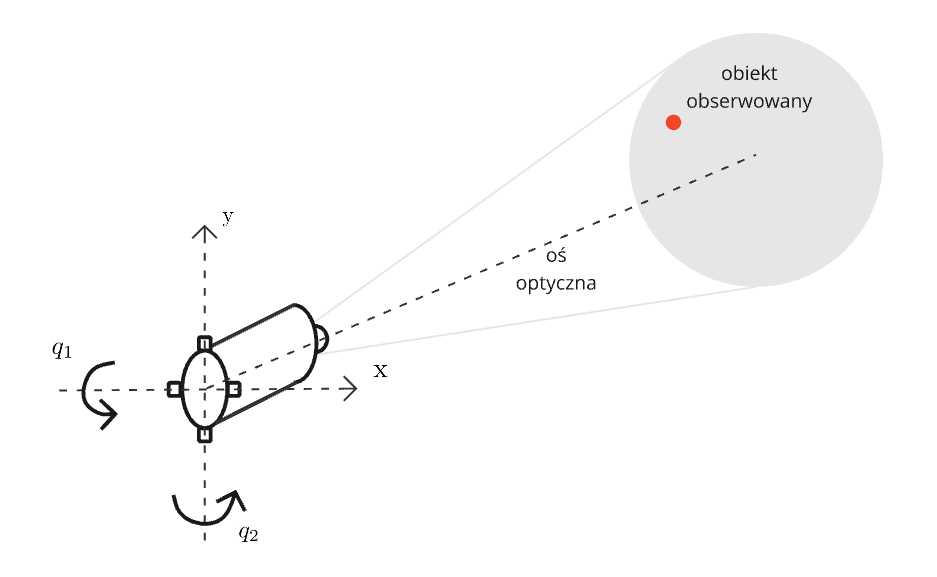
\includegraphics{testy/schematpogladowy.png}}
    \caption{Schemat poglądowy stanowiska badawczego}
    \label{fig:podglad5}
\end{figure}

\noindent Kąty te można interpretować jako dwa kąty Eulera opisujące orientację układu lokalnego względem układu podstawowego. Orientację tę można wyrazić za pomocą macierzy transformacji opisanych następująco: 

\begin{equation}
R_x(q_1) = 
\begin{bmatrix}
1 & 0 & 0\\
0 & \cos(q_1) & -\sin(q_1)\\
0 & \sin(q_1) & \cos(q_1)\\
\end{bmatrix},\ 
R_y(q_2) = 
\begin{bmatrix}
\cos(q_2) & 0 & \sin(q_2)\\
0 & 1 & 0 &\\
-\sin(q_2) & 0 & \cos(q_2)\\
\end{bmatrix},
\end{equation}
%
gdzie $R_x(q_1)$ i $R_y(q_2)$ określają elementarne obroty wokół osi X i Y układu lokalnego, przy czym kąty wyrażone są odpowiednio przez $q_1$ i $q_2$.
%\begin{center}
%\textit{Rotacja wokół %osi Y o $q_2$}
%\[
%\]}
%\textit{Rotacja wokół osi X o $q_1$}
Wypadkowa orientacja układu lokalnego wynika z następującego złożenia tych dwóch obrotów
%
\begin{equation}\label{eq:R_def}
R=R_x(q_1) \cdot R_y(q_2) =
\begin{bmatrix}
\cos(q_2) & 0 & \sin(q_2)\\
\sin(q_1) \sin(q_2) & \cos(q_1) & -\sin(q_1) \cos(q_2)\\
-\cos(q_1) \sin(q_2) & \sin(q_1) & \cos(q_1) \cos(q_2)\\
\end{bmatrix}.
\end{equation}
%
%określających obrót poszczególnych osi możliwe jest określenie położenia punktu w przestrzeni w odniesieniu do układu bazowego.
Przyjmując, że pozycja pewnego punktu w układzie lokalnym o orientacji początkowej zgodnej z układem podstawowym opisywana jest przez wektor $d=[d_x\ d_y\  d_z]^T\in\mathbb{R}^3$, to po wykonaniu obrotu opisanego przez \eqref{eq:R_def} jego pozycja w układzie podstawowym spełnia zależność
%
\begin{equation}
d^{'}=R \cdot d.    
\end{equation}
%
%
%wynosi $p^{T}=[p_x, p_y, p_z]$ i tym samym opisuje wektor kierunku $d^{T}=[d_x, d_y, d_z]$
%\textit{Macierz transformacji aktualnego położenie punktu względem układu}
%\noindent Po wyznaczeniu macierzy rotacji możemy obliczyć nowy wektor kierunku $p^'$ po rotacji oraz wyznaczyć nowe współrzędne punktu obserwowanego przez teleskop
%$d^{'}=R \cdot d$
%$$p^{'T}=[p_{x0}+d^{'}_{x}, p_{y0}+d^{'}_{y}, p_{z0}+d^{'}_{z}]$$

\noindent W tej pracy w roli elementu pozycjonującego  wykorzystano konstrukcję mechaniczną, której układ kinematyczny odpowiada przypadkowi zilustrowanemu na Rys.\ref{fig:podglad5}. Na Rys. \ref{fig:lkjlkjlkj} przedstawiono dwa widoki izometryczne konstrukcji, a na rys. \ref{fig:stan} jego widok rzeczywisty. 

\begin{figure}[!htb]
    \centering
    \resizebox{15cm}{!}{
    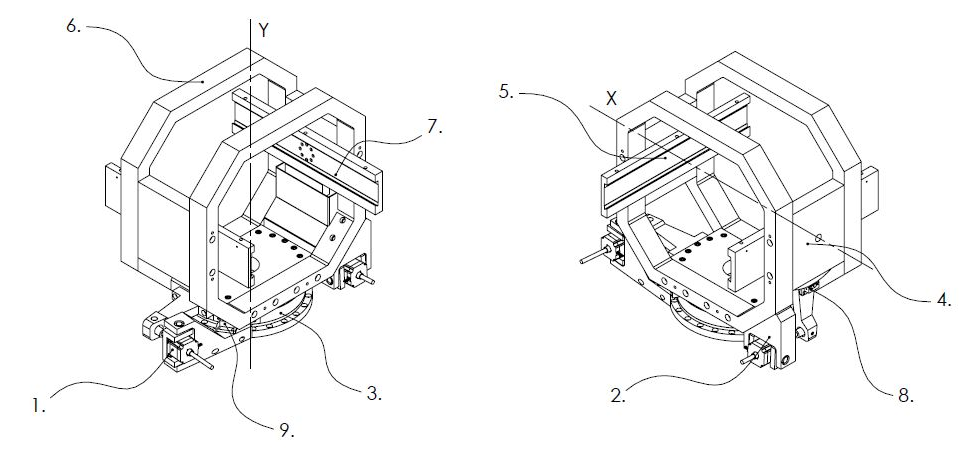
\includegraphics{pictures/lkjlkjlkj.png}}
    \caption{Widoki izometryczne stanowiska \cite{konstrukcja}}
    \label{fig:lkjlkjlkj}
\end{figure}

\begin{center}
    \begin{minipage}{0.45\textwidth}
        1. Układ napędowy osi X\\
        2. Układ napędowy osi Y\\
        3. Zespół łożyskowania osi Y\\
        4. Zespół łożyskowania osi X - węzeł napędowy\\
        5. Zespół łożyskowania osi X - węzeł swobodny
    \end{minipage}%
    \hspace{0.05\textwidth} 
    \begin{minipage}{0.45\textwidth}
        6. Klatka zespalająca\\
        7. Uchwyty mocujące teleskopy - złącze uniwersalne\\
        8. Układ pomiarowy obrotu osi X\\
        9. Układ pomiarowy obrotu osi Y
    \end{minipage}
\end{center}

\vspace{0.5cm}

\begin{figure}[!htb]
    \centering
    \resizebox{10cm}{!}{
    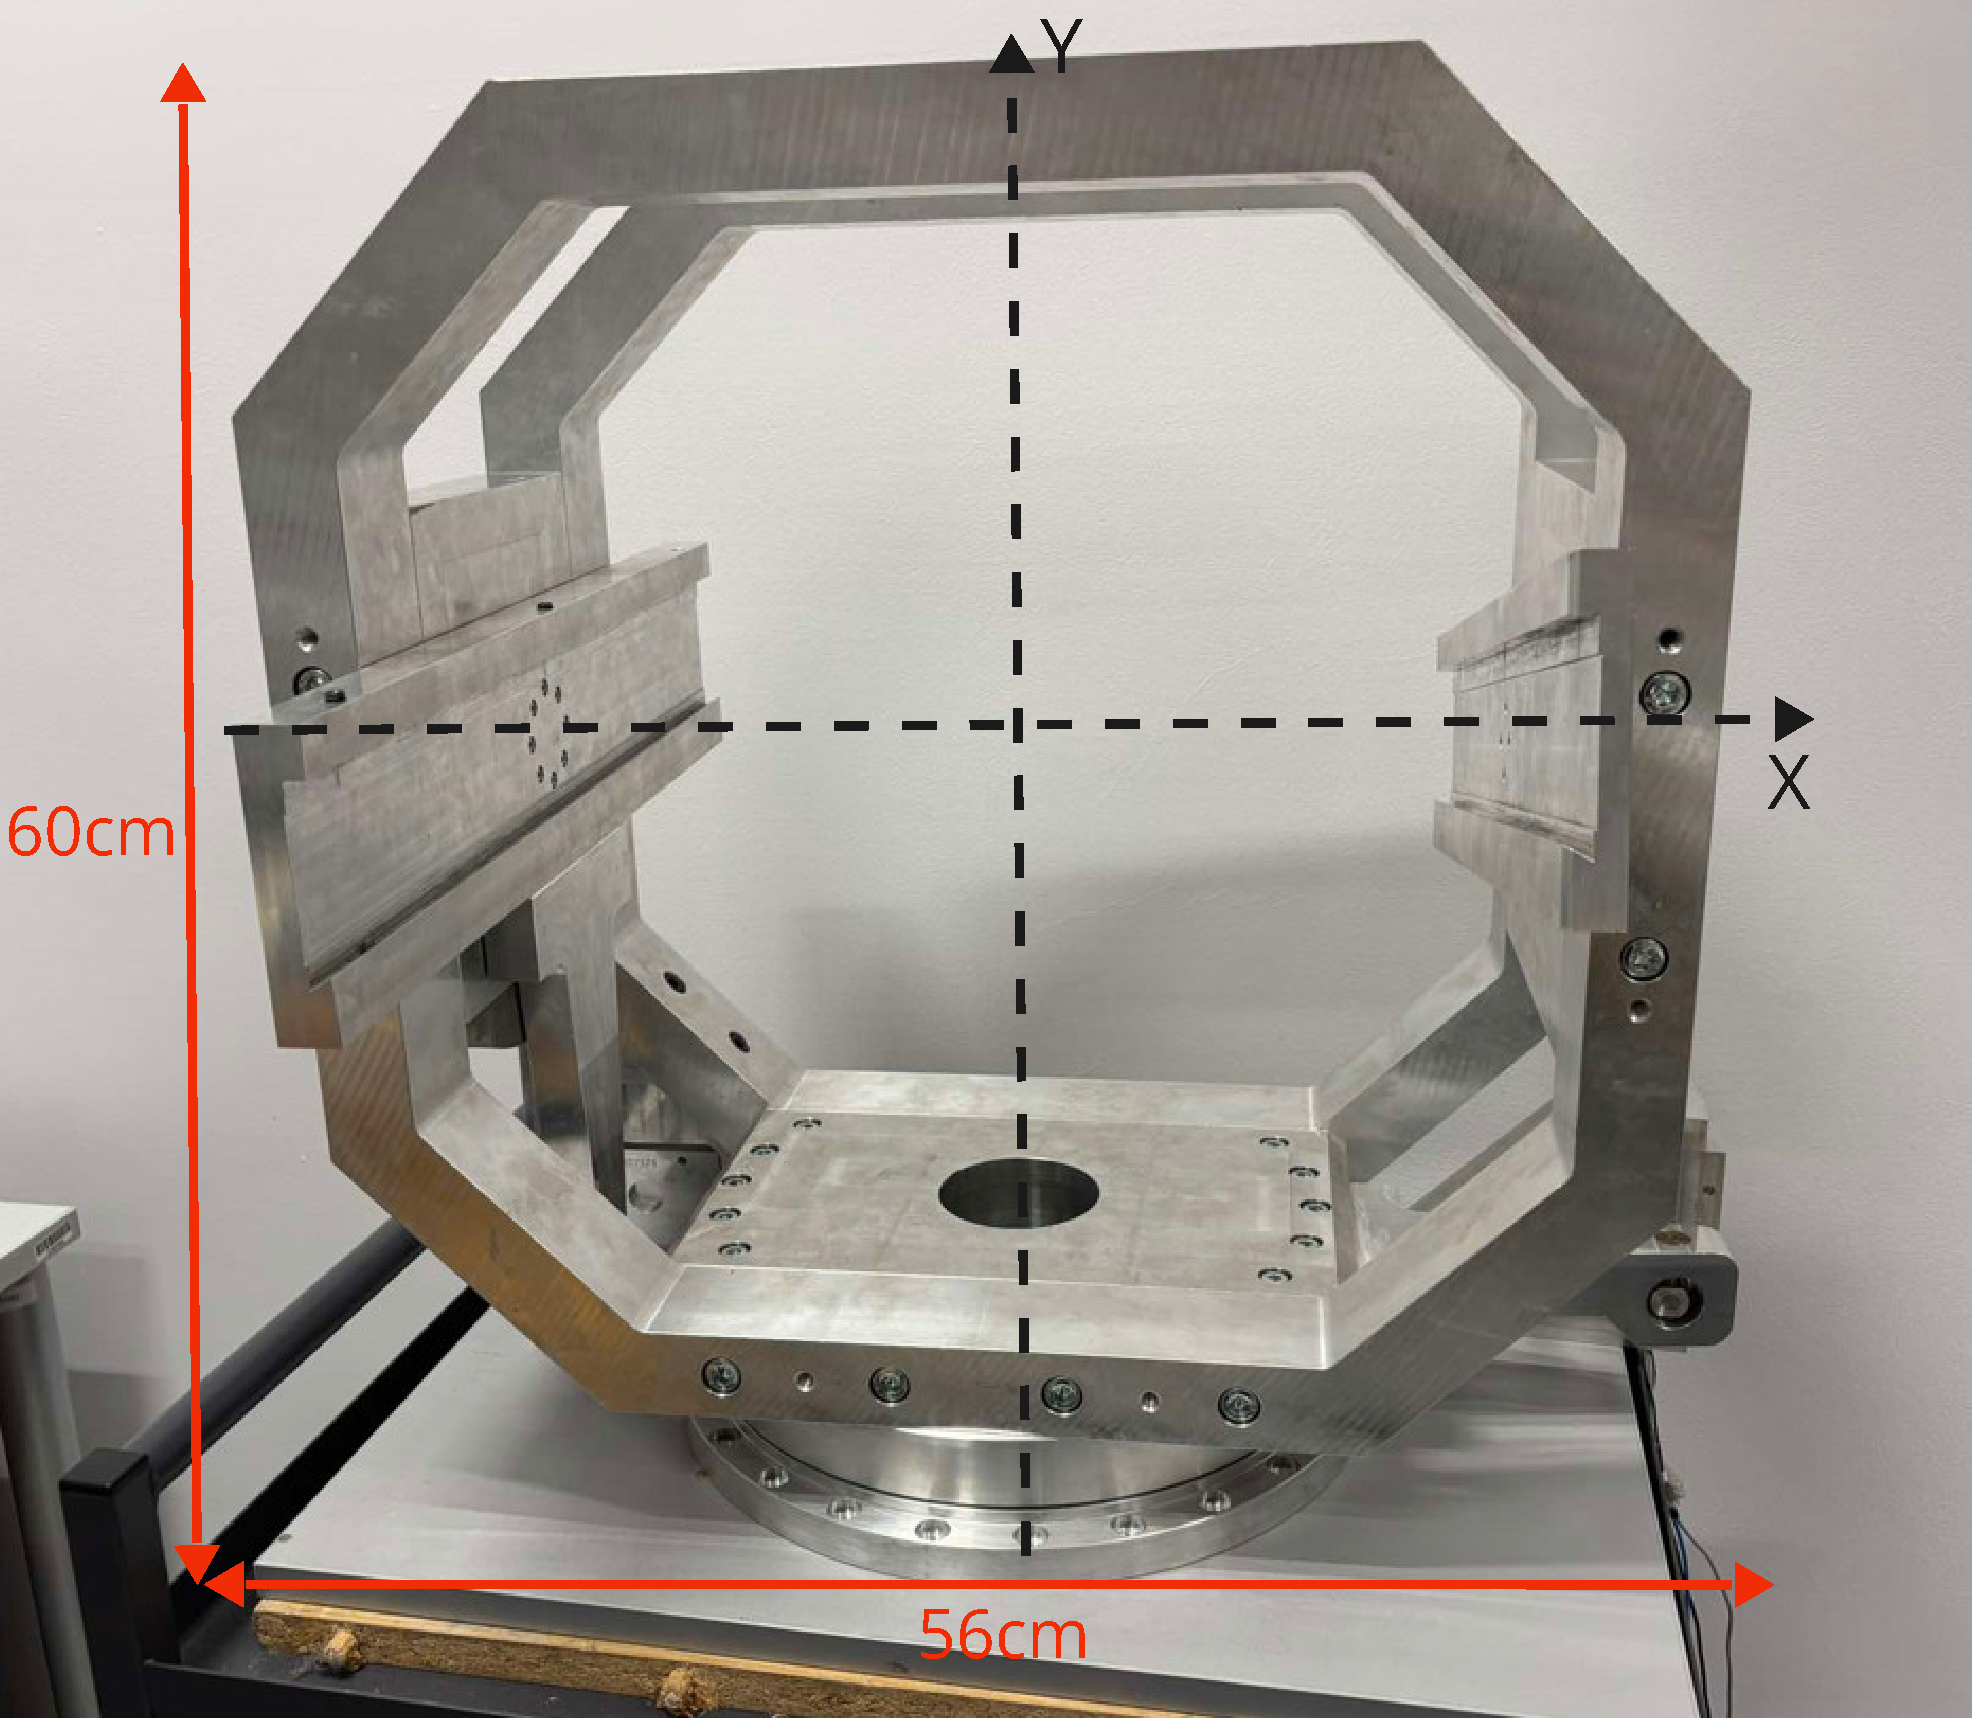
\includegraphics{pictures/Inżynierka (13).pdf}}
    \caption{Stanowisko w sali laboratoryjnej o wymiarach 56cm x 50cm x 60cm}
    \label{fig:stan}
\end{figure}

\vspace{1cm}

\begin{figure}[!htb]
    \centering
    \resizebox{10cm}{!}{
    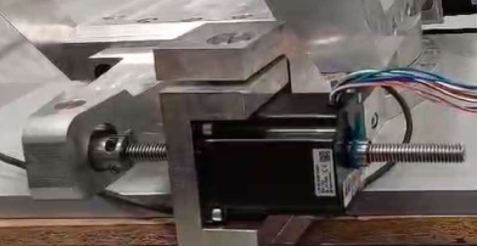
\includegraphics{pictures/przekladnia.png}}
    \caption{Silnik krokowy z przekładnią śrubową}
    \label{fig:śruba}
\end{figure}

\vspace{1cm}

\noindent Widoczne na rys. \ref{fig:śruba} połączenie z przekładnią śrubową silnika krokowego zapewnia precyzyjną konwersję ruchu obrotowego na liniowy umożliwiając uzyskanie bardzo dokładnego przesunięcia. Jest to spowodowane obrotem śruby, która porusza się z uwagi na oddziałujące na nią sprzęgło uzależnionego od połączonego z nim napędu. Dzięki właściwości samohamowności śruby trapezowej układ nie wymaga ciągłego podtrzymywania pozycji, a duża siła przesuwu jest osiągana nawet przy niewielkim momencie obrotowym silnika.

\newpage
